\section{Introduccion y Teoria}
\subsection{Introduccion}
En el presente trabajo utilizaremos redes neuronales artificiales entrenadas con retropropagacion de errores (backpropagation) para modelar dos problemas distintos. La idea sera entrenar la red con informacion contenida en dos bases de datos.

El primer problema consiste en dada unas muestras de tumores de mamas, poder calificar si un tumor corresponde o no con tumores \textbf{malignos} o \textbf{benignos}.

El segundo problema dada una muestra con ciertos atributos de edificios, tales como superficie total u oritancion, podremos precedir la \textbf{cantidad de energia necesaria para calefaccionar y refrigerar los edificios}.

Se espera entonces que utilizando lo que vimos en la materia podamos desarrollar redes que resuelvan correctamente ambos problemas. 

Adicionalmente se espera hacer un analisis y experimentacion del funcionamiento de un perceptron multicapa con retropropagacion de errores.

\subsection{Introduccion Teorica}
La idea principal del perceptron multicapa es utilizar el paradigma de aprendizaje supervisado con un algoritmo de correccion de errores. Es una red neuronal artificial formada por multiples capas, esto le permite resolver problemas que no son linealmente separables, lo cual es la principal limitación del perceptron simple.

\begin{center}
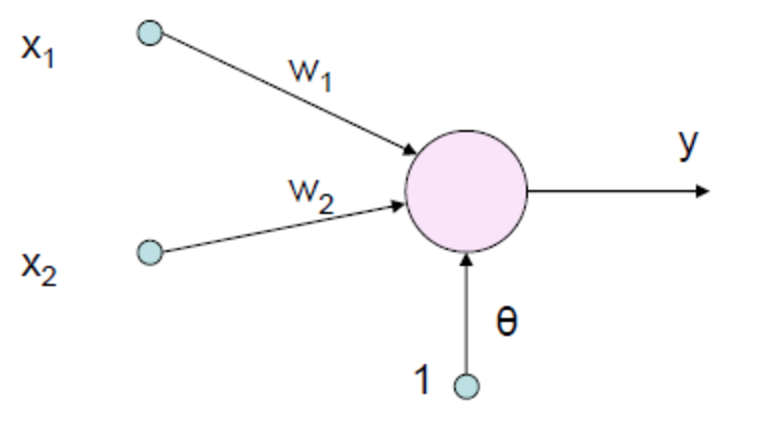
\includegraphics[width=0.25\textwidth]{img/psimple}
\end{center}

El aprendizaje supervisado se basa en un entrenamiento en el cual se provee al sistema con informacion de las entradas y de igual forma se proveen las salidas esperadas para cada entrada en particular.

Intuitivamente, el perceptron multicapa permite aproximar funciones, categorizar y encontrar patrones.

\begin{center}
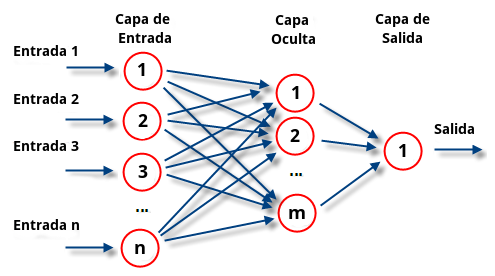
\includegraphics{img/pmulticapa}
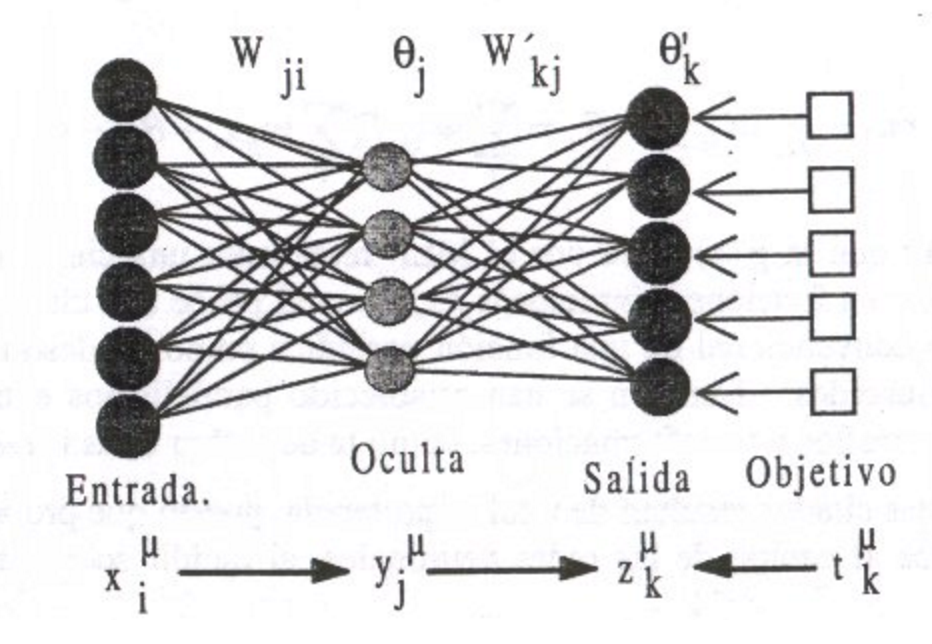
\includegraphics[width=0.35\textwidth]{img/pmulticapa2}
\end{center}

Las neuronas de la capa oculta usan como regla de propagacion la suma ponderada de las entradas con los pesos sinápticos $w_{ij}$ y sobre esa suma ponderada se aplica una funcion de transferencia de tipo sigmoide, que es acotada en respuesta.

\newpage
Grafico de funcion sigmoide:

\begin{center}
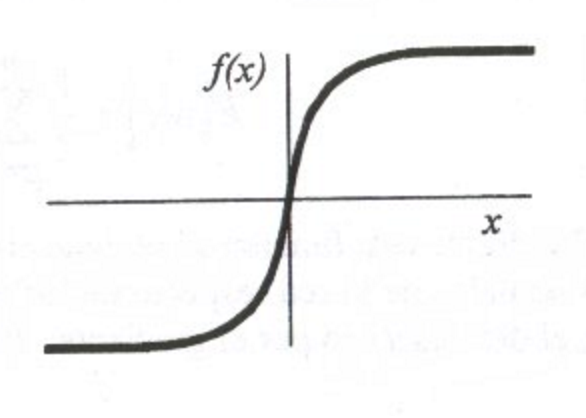
\includegraphics[width=0.30\textwidth]{img/sigmoide}
\end{center}

Sobre el aprendizaje, para este se suele usar en este tipo de redes recibe el nombre de backpropagation. Como funcion de coste global, se usa el error cuadratico medio. Es decir, que dado un par ($x_k$, $d_k$) correspondiente a la entrada k de los datos de entrenamiento y salida deseada asociada se calcula la cantidad.

Por otro lado, las capas pueden clasificarse en tres tipos:

\begin{enumerate}
\item \textbf{Capa de entrada:} Constituida por aquellas neuronas que introducen los patrones de entrada en la red. 
\item \textbf{Capas ocultas:} Formada por aquellas neuronas cuyas entradas provienen de capas anteriores y cuyas salidas pasan a neuronas de capas posteriores.
\item \textbf{Capa de salida:} Neuronas cuyos valores de salida se corresponden con las salidas de toda la red.
\end{enumerate}


En general la estructura de una neurona se puede representar de la siguiente manera:

\begin{center}
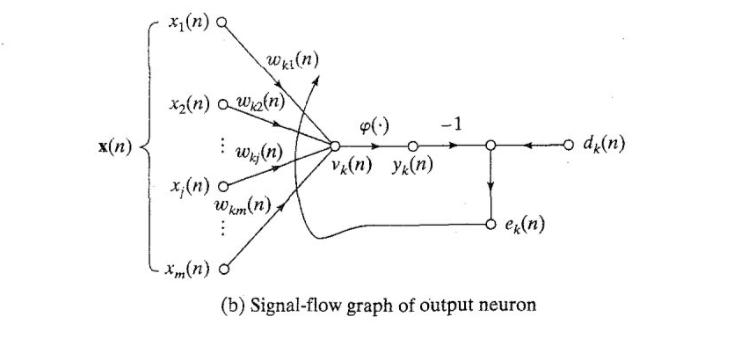
\includegraphics[width=0.6\textwidth]{img/neurona}
\end{center}

Podemos observar como los elementos mas importantes al vector de entrada de la neurona $(x_1,...,x_m)$, a los pesos correspondientes como $w_{ij}$, a la funcion de activacio y al elemento de salida. A partir de esta estructura basica la neurona puede mapear las entradas para obtener a la salida una respuesta deseada que pudiera pertenecer a alguna funcion a de terminar.


La funcion de activacion trata de simular el mecanismo que realiza el sistema de neuronas en el cerebro, que se basa en la exitacion de las neuronas hasta un cierto punto en el cual se pasa un umbral en el que dicha neurona dispara la informacion que le corresponde. Entre las diferentes funciones de activacion podemos encontrar la sigmoide.


Por otro lado el perceptron cuenta con un coeficiente de entrenamiento que indica que tanto varian los pesos entre iteracion e iteracion, por lo cual indica que tan lento o rapido la red se entrena.